\documentclass[10pt,a4paper, margin=1in]{article}
\usepackage{fullpage}
\usepackage{amsfonts, amsmath, pifont}
\usepackage{amsthm}
\usepackage{graphicx}
\usepackage{float}
\usepackage{mathtools} 
\usepackage{extarrows}

\usepackage{tkz-euclide}
\usepackage{tikz}
\usepackage{pgfplots}
\pgfplotsset{compat = newest}

\usepackage{geometry}
 \geometry{
 a4paper,
 total={210mm,297mm},
 left=10mm,
 right=10mm,
 top=10mm,
 bottom=10mm,
 }
 % Write both of your names here. Fill exxxxxxx with your ceng mail address.
 \author{
  Adıgüzel, Gürhan İlhan\\
  \texttt{e2448025@ceng.metu.edu.tr}
  \and
  İçen, Anıl\\
  \texttt{e2448488@ceng.metu.edu.tr}
}

\title{CENG 384 - Signals and Systems for Computer Engineers \\
Spring 2023 \\
Homework 4}
\begin{document}
\maketitle


\noindent\rule{19cm}{1.2pt}

\begin{enumerate}

\item %write the solution of q1
    \begin{enumerate}   
    % Write your solutions in the following items.
    \item %write the solution of q1a
        \[  H(jw) = \frac{jw-1}{jw+1} \]
        \[ \frac{Y(jw)}{X(jw)} = \frac{jw-1}{jw+1}\]
        \[ jwX(jw)-X(jw) = jwY(jw) + Y(jw)\]
        \[ x'(t)-x(t) = y'(t) - y(t)\]
        
    \item %write the solution of q1b
        \[ H(jw) = \frac{jw-1}{jw+1} \]   
        \[ H(jw) = 1 + \frac{-2}{jw+1} \] 
        \[ h(t) = (\delta(t) -2e^{-1t})u(t)\]
        
    \item %write the solution of q1c
        \[ X(jw) = \frac{1}{jw+2} \]
        \[ Y(jw) = X(jw).H(jw) \]
        \[ Y(jw) = \frac{1}{jw+2} . \frac{jw-1}{jw+1}\]
        \[ Y(jw) = \frac{3}{jw+2} - \frac{2}{jw+1}\]
        \[ y(t) = (3e^{-2t} - 2e^{-t})u(t)\]
        \begin{align*}
            \begin{tikzpicture}
                \begin{axis}[
                    xmin = 0, xmax = 10,
                    ymin = -1.2, ymax = 1.2,
                    ]
                    \addplot[domain = 0:30,samples = 200,] {(3*exp(-2*x))-(2*exp(-x))};
                \end{axis}
            \end{tikzpicture}
        \end{align*}
        \[ y(t) = (3e^{-2t} - 2e^{-t})u(t) \]
        
    \item %write the solution of q1d

        \begin{center}
	\tikzset{%
		block/.style    = {draw, thick, rectangle, minimum height = 3em,
			minimum width = 3em},
		sum/.style      = {draw, circle, node distance = 2cm}, % Adder
		input/.style    = {coordinate}, % Input
		output/.style   = {coordinate} % Output
	}
	% Defining string as labels of certain blocks.
	\newcommand{\suma}{\Large$+$}
	\newcommand{\inte}{$\displaystyle \int$}
	\newcommand{\derv}{\huge$\frac{d}{dt}$}
	
\begin{tikzpicture}[auto, thick, node distance=3cm, >=triangle 45]
	\draw
	% Drawing the blocks of the filter:
	node at (0, 0) [input] (inp) {\Large \textopenbullet}
	node [sum, right of=inp] (sum1) {\suma}
	node [sum, right of=sum1] (sum2) {\suma}
	node [block, right of=sum2] (int) {\inte}
	node [output, right of=int] (out) {}
	node [output, right of=out] (out2) {\Large \textopenbullet}
	node [output, below of=out] (temp1) {}
	node [output, below of=sum2] (temp2) {}
	% Drawing the block for derivative:
	node [block, below of=inp] (derivative) {$\frac{d}{dt}$}
	;
	% Connecting the nodes:
	\draw[->](inp) -- node{$-x(t)$} (sum1);
	\draw[->](sum1) -- (sum2);
	\draw[->](sum2) -- (int);
	\draw[-](int) -- (out);
	\draw[->](out) -- node{$y(t)$} (out2);
	\draw[-](out) -- (temp1);
	\draw[->](temp2) -- (sum2);
	\draw[->](inp) -- (derivative);
	\draw[->](derivative) -| node[pos=0.95] {$x'(t)$} (sum1);
\end{tikzpicture}

\end{center}
\end{enumerate}

\item %write the solution of q2  
    \begin{enumerate}
    % Write your solutions in the following items.
    \item %write the solution of q2a
        \[ e^{jw}Y(e^{jw}) - \frac{1}{2}Y(e^{jw}) = e^{jw}X(jw)\]
        \[ Y(jw)(e^{jw} - \frac{1}{2}) = e^{jw}X(jw)\]
        \[ \frac{Y(jw)}{X(jw)} = \frac{e^{jw} - \frac{1}{2}}{e^{jw}}\]
        \[ H(e^{jw}) = 1 - \frac{1}{2e^{jw}}\]
        
    \item %write the solution of q2b
        \[ H_1(e^{jw}) = 1 \xleftrightarrow{FT}  h_1[n]= \delta[n] \] 
        \[ H_2(e^{jw}) = \frac{1}{2e^{jw}} \xleftrightarrow{FT} h_2[n]  = - \frac{1}{2}\delta[n-1]\]
        \[ h[n] = \delta[n] - \frac{1}{2}\delta[n-1] \]
        
    \item %write the solution of q2c
        \[ y[n] = x[n]*h[n] \]
        \[ y[n] = x[n] - \frac{1}{2}x[n-1] \]
        \\ When $x[n] = \left( \frac{3}{4}\right)^n u[n]$:
        \[ y[n] = \left( \frac{3}{4}\right)^n u[n] - \frac{1}{2} \left( \frac{3}{4}\right)^{n-1} u[n-1]\]
\end{enumerate}

\item %write the solution of q3
    \begin{enumerate}
    % Write your solutions in the following items.
    \item %write the solution of q3a
        \[ H(jw) = H_1(jw) . H_2(jw)\]
        \[ H(jw) = \frac{1}{jw+1} . \frac{1}{jw+2}\]
        \[ \frac{Y(jw)}{X(jw)} = \frac{1}{(jw)^2 + 3(jw) + 2}\]
        \[ (jw)^2Y(jw) + 3(jw)Y(jw) + 2Y(jw) = X(jw)\]
        \[ (jw)^2Y(jw) \xleftrightarrow{FT} y''(t) \]
        \[ 3(jw)Y(jw) \xleftrightarrow{FT} 3y'(t) \]
        \[ 2Y(jw) \xleftrightarrow{FT} 2y(t) \]
        \[ X(jw) \xleftrightarrow{FT} x(t)\]
        \[ y''(t) + 3y'(t) + 2y(t) = x(t)\]
        
    \item %write the solution of q3b
        \[ H(jw) = \frac{1}{jw+1} . \frac{1}{jw+2}\]
        \[ H(jw) = \frac{1}{jw+1} - \frac{1}{jw+2}\]
        \[ H_3(jw) = \frac{1}{jw+1} \xleftrightarrow{FT} h_1(t) = e^{-t}u(t)\]
        \[ H_4(jw) = \frac{1}{jw+2} \xleftrightarrow{FT} h_2(t) = e^{-2t}u(t)\]
        \[ h(t) = h_1(t) + h_2(t)\]
        \[ h(t) = (e^{-t} + e^{-2t})u(t)\]
        
    \item %write the solution of q3c
        \[ H(jw) = \frac{1}{jw+1} - \frac{1}{jw+2}\]
        \[ \frac{Y(jw)}{X(jw)} = \frac{1}{jw+1} - \frac{1}{jw+2}\]
        \[ Y(jw) = \frac{1}{jw+1}X(jw) - \frac{1}{jw+2}X(jw)\]
        \\ When $X(jw) = jw$ :
        \[ Y(jw) =\frac{jw}{jw+1} - \frac{jw}{jw+2} \]
        \[ Y(jw) = \left( 1-\frac{1}{jw+1} \right) - \left(1 - \frac{2}{jw+2} \right)\]
        \[ Y(jw) = \frac{2}{jw+2} - \frac{1}{jw+1}\]
        \[ y(t) = (2e^{-2t} - e^{-t})u(t)\]
\end{enumerate}

\item %write the solution of q4
    \begin{enumerate}   
    % Write your solutions in the following items.
    \item %write the solution of q4a
        \[ H(e^{jw}) = H_1(e^{jw}) + H_2(e^{jw})\]
        \[ H(e^{jw}) = \frac{3}{3+e^{-jw}} + \frac{2}{2+e^{-jw}}\]
        \[ \frac{Y(e^{jw})}{X(e^{jw})} = \frac{5e^{-jw} + 12}{e^{-2jw} + 5e^{-jw} + 6}\]
        \[ e^{-2jw}Y(e^{jw}) + 5e^{-jw}Y(e^{jw}) + 6Y(e^{jw}) = 5e^{-jw}X(e^{jw}) + 12X(e^{jw}) \]
        \[ e^{-2jw}Y(e^{jw}) \xleftrightarrow{FT} y[n-2]\]
        \[ 5e^{-jw}Y(e^{jw}) \xleftrightarrow{FT} 5y[n-1]\]
        \[ 6Y(e^{jw}) \xleftrightarrow{FT} 6y[n]\]
        \[ 5e^{-jw}X(e^{jw}) \xleftrightarrow{FT} 5x[n-1]\]
        \[ 12X(e^{jw}) \xleftrightarrow{FT} 12x[n]\]
        \[ y[n-2] + 5y[n-1] + 6y[n] = 5x[n-1] + 12x[n]\]
        
    \item %write the solution of q4b
        \[ H(e^{jw}) = \frac{1}{1+\frac{1}{3}e^{-jw}} + \frac{1}{1+\frac{1}{2}e^{-jw}}\]
        
    \item %write the solution of q4c
        \[ h[n] = h_1[n] + h_2[n]\]
        \[ H_1(e^{jw}) = \frac{1}{1+\frac{1}{3}e^{-jw}} \xleftrightarrow{FT} h_1[n] = \left( \frac{-1}{3}\right)^n u[n] \]
        \[ H_2(e^{jw}) = \frac{1}{1+\frac{1}{2}e^{-jw}} \xleftrightarrow{FT} h_2[n] = \left( \frac{-1}{2}\right)^n u[n] \]
        \[ h[n] = \left( \left( \frac{-1}{2}\right)^n + \left( \frac{-1}{3}\right)^n \right) u[n]\]
\end{enumerate}

\newpage
\item %write the solution of q5
    \begin{enumerate}
         \begin{verbatim}
            import numpy as np
            import matplotlib.pyplot as plt
            from scipy.io import wavfile
            
            def fft(signal):
                N = len(signal)
                if (N <= 1):
                    return signal
                even = fft(signal[::2])
                odd = fft(signal[1::2])
                T = [np.exp(-2j * np.pi * i / N) * odd[i] for i in range(N // 2)]
                return [even[i] + T[i] for i in range(N // 2)] 
                        +[even[i] - T[i] for i in range(N // 2)]
            
            def ifft(signal):
                N = len(signal)
                conjugate_signal = np.conjugate(signal)
                fft_signal = fft(conjugate_signal)
                return np.conjugate(fft_signal) / N
            
            
            sample_rate, encoded_signal = wavfile.read('encoded.wav')
            
            
            encoded_data = fft(encoded_signal)
            
            
            positive_freq = encoded_data[:len(encoded_data)//2]
            negative_freq = encoded_data[len(encoded_data)//2:]
            
            
            reversed_positive_freq = positive_freq[::-1]
            reversed_negative_freq = negative_freq[::-1]
            
            
            reversed_fft = np.concatenate((reversed_positive_freq, reversed_negative_freq))
            
            # Perform IFFT on the reversed FFT
            decoded_data = ifft(reversed_fft).real
            
            # Convert the decoded signal to integer type
            decoded_data = np.int16(decoded_data)
            
            # Save the decoded audio as "decoded.wav" file
            wavfile.write('decoded.wav', sample_rate, decoded_data)
            
            plt.figure(figsize=(10, 6))
            plt.subplot(2, 1, 1)
            plt.magnitude_spectrum(encoded_data, Fs=sample_rate, scale='dB')
            plt.title('Encoded Signal')
            plt.subplot(2, 1, 2)
            plt.magnitude_spectrum(decoded_data, Fs=sample_rate, scale='dB')
            plt.title('Decoded Signal')
            plt.tight_layout()
            plt.show()
            
            plt.figure(figsize=(10, 6))
            plt.subplot(2, 1, 1)
            plt.plot(encoded_data)
            plt.title('Encoded Signal')
            plt.subplot(2, 1, 2)
            plt.plot(decoded_data)
            plt.title('Decoded Signal')
            plt.tight_layout()
            plt.show()
        \end{verbatim}
    \end{enumerate}
    $ \hspace{50} $ The message is : "I HAVE A DREAM".
    \begin{figure}[htp] \centering{
        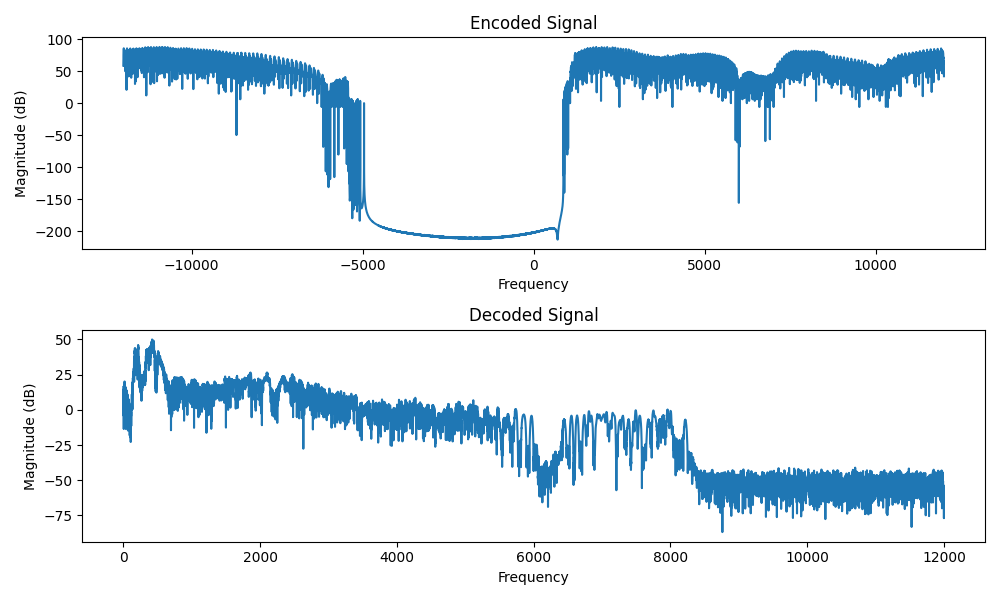
\includegraphics[scale=0.55]{hw4/magnitude_spectrum.png}}
        \caption{Frequency Domain Magnitude of Encoded and Decoded Signal}
    \end{figure}
    \begin{figure}[htp] \centering{
        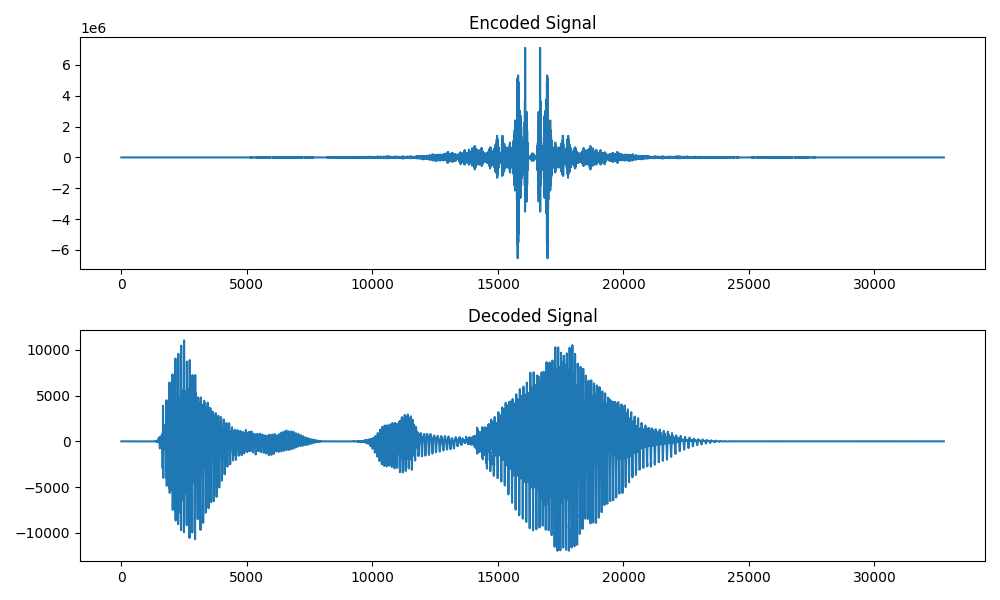
\includegraphics[scale=0.55]{hw4/signal.png}}
        \caption{Time Domain Magnitude of Encoded and Decoded Signal}
    \end{figure}
\end{enumerate}
\end{document}

